گرامر سوال:

\begin{align*}
	S&\rightarrow A \\
	A&\rightarrow By|xx \\
	B&\rightarrow x|yBx \\
\end{align*}


ترنزیشن دیاگرم
$LR(0)$
مربوط به گرامر فوق:

\qquad\qquad\qquad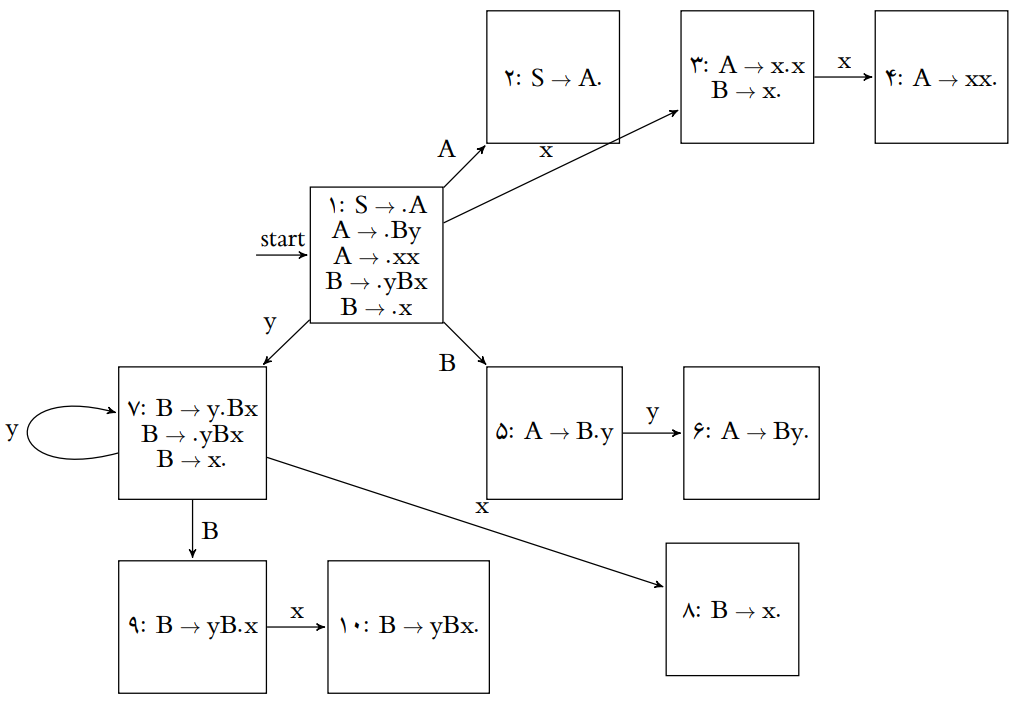
\includegraphics[width=0.7\linewidth]{figs/3.png}



\subsubsection*{الف}

در یکی از قواعد استیت‌ شماره 3، 
$\bullet$
به انتها رسیده و در باقی قواعد می‌توان با ترمینال $x$ حرکت کرد. چون که $x$ عضو $follow(x)$ است پس در خانه‌ی  $(3,x)$ نداخلی از نوع $shift-reduce$ داریم.

\setLTR
$
shift 4 / reduce 4
$
\setRTL

پس گرامر ما نوع $SLR(1)$ نیست.

\subsubsection*{ب}

مجموعه‌ی $Follow$ها عبارتند از:

\begin{align*}
	Follow(S)&=\{\$\} \\
	Follow(A)&=\{\$\} \\
	Follow(B)&=\{x,y\} 
\end{align*}
\pagebreak

\subsubsection*{ج}
مجموعه 
$Look-Ahead$
های دیاگرام فوق:

\setLTR
$
{LA_{state2} = \{\$\}} \qquad {LA_{state3} = \{y\}} \qquad {LA_{state4} = \{\$\}} \\
{LA_{state6} = \{\$\}} \qquad {LA_{state7} = \{x,y\}} \qquad {LA_{state8} = \{x\}} \qquad {LA_{state10} = \{x,y\}} 
$
\setRTL

\subsubsection*{د}
جدول را تشکیل می‌دهیم، اگر تداخلی وجود نداشت این گرامر 
$LALR(1)$
است و اگر تداخلی وجود داشت گرامر 
$LALR(1)$
نیست:

\qquad\qquad\qquad\qquad\qquad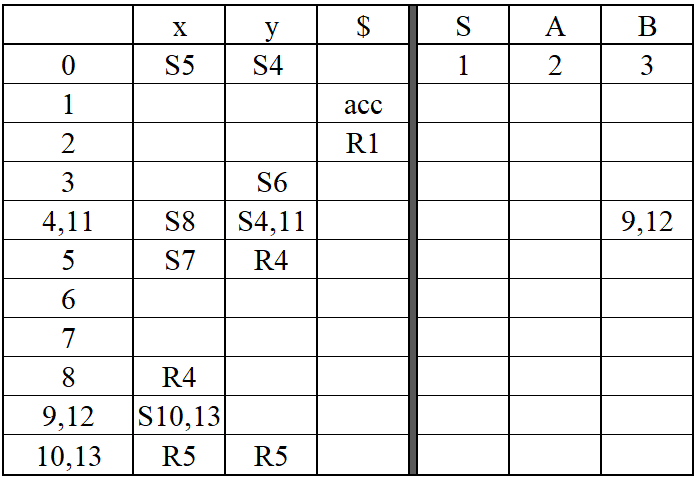
\includegraphics[width=0.5\linewidth]{figs/5.png}

پس گرامر فول از نوع 
$LALR(1)$
است.
\subsubsection*{ه}

با توجه به بخش قبلی، چون گرامر ما 
$LALR(1)$
است، پس 
$LA(1)$
هم است.




$\\ \\ \\ \\$
ترنزیشن دیاگرم
$LR(1)$
مربوط به گرامر فوق:

\qquad\qquad\qquad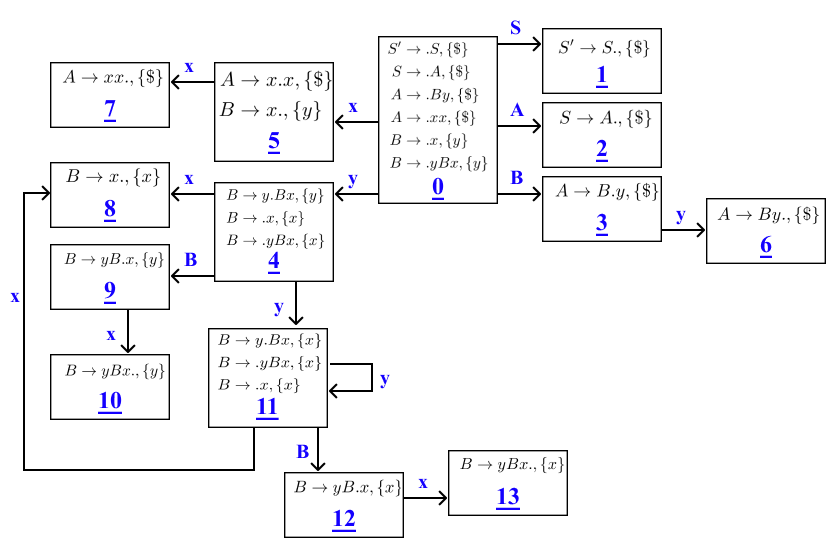
\includegraphics[width=0.7\linewidth]{figs/4.png}


















